\chapter{Research Results}
\begin{multicols}{2}
      \section{Research Topic}
      In research, it is paramount to have the formulation of a clear research topic, research main question,
      and research sub-questions. The main question serves as the focal point around which the research revolves,
      encapsulating the primary objective or purpose of the study.
      The following main research question will be used throughout the research:
      \begin{center}
            \textit{"How can Quality ICT B.V. effectively integrate and leverage SentinelOne EDR platform
                  for continuous cybersecurity monitoring?"}
      \end{center}
      The research sub-questions are then used to function as a pathway that dissects the main
      question into smaller, more manageable components, which can then be addressed individually. This approach
      allows for a more comprehensive and in-depth analysis of the research topic, ensuring that all relevant
      aspects are covered and that the research is conducted in a systematic and organized manner.
      This research main question is therefore expanded in the following research sub-questions:
      \begin{itemize}
            \item What is the current situation of the \acrshort{qaas} app of \acrlong{qict} \acrshort{bv}?
            \item How can SentinelOne be integrated into the \acrshort{qaas} app environment, while still
                  utilizing their key features and capabilities in context of cyber-threat detection and
                  remote \acrshort{it} infrastructure management?
            \item What are the most suitable visualization techniques for displaying the data processed and
                  received by other Security Threat Platforms to ensure clear and insightful representation
                  of threats detected by SentinelOne \acrshort{api}?
            \item How should the QaaS app respond in the event of a cybersecurity incident detected through
                  the utilization of SentinelOne technologies and packages?
      \end{itemize}
      \section{Research Methodology}
      In this research, different research methods have been used to answer the research questions. This research
      will be based on the six \acrshort{ict} research methods defined by HBO-I (\cite{ictresearchmethods}). A
      research method for each sub-question is then defined along with how the results are considered valid and
      reliable:
      \subsection{Method of Data Collection}
      \begin{itemize}[label=-]
            \item Sub-question \#1: desk research of Literature Study will be conducted, with the goal of creating
                  infrastructure information that displays the structure of the \acrshort{qaas} app and all of its
                  dependencies. Furthermore, Interview with key stakeholders involved in the  development, maintenance,
                  and usage of the \acrshort{qaas} app will be conducted to gain insights into the current situation
                  of the app.
            \item Sub-question \#2: Literature Study on various articles on the Internet, interviews, expert reviews,
                  and requirement elicitation techniques such as use case analysis and user stories. Analysis on the
                  current \acrshort{qaas} app and its \acrshort{api} monitoring capabilities.
            \item Sub-question \#3: technical evaluations of SentinelOne's capabilities and \acrshort{api}s will
                  be conducted, the \acrshort{api} documentation and integration guideline will be read and review
                  with Literature Study method and case studies of similar integrations. Requirements from the
                  cybersecurity experts from the \acrshort{qict} department responsible for SentinelOne's technical
                  support will be gathered and analyzed. Furthermore, Prototyping with proof-of-concept prototypes
                  on a test environment will be conducted to test different integration scenarios, assess feasibility,
                  identify potential challenges, refine the approach, and evaluate the performance of the integration.
            \item Sub-question \#4: research into existing visualization techniques for \acrshort{xml} and
                  \acrshort{json} data, especially the data coming from SentinelOne \acrshort{api} through Literature
                  Study. Analyze existing data visualization tools and platforms that are available in Flutter and
                  Firebase. Gather requirements from project stakeholders regarding data visualization preferences and
                  usability, and do data analysis and usability testing.
      \end{itemize}
      \subsection{Selected Measuring Instruments}
      \begin{itemize}[label=-]
            \item Sub-question \#1: structured interview guide, document report checklist analysis and review,
                  observation, analysis tools for codebase and logs, and quite possibly supplemented by surveys
                  or questionnaires.
            \item Sub-question \#2: document analysis tools for literature review. Structured questionnaires for
                  requirement interviews regarding functionality rating scale and compare the response against
                  industry standards and best practices. Observation of existing \acrshort{api} monitoring tools.
                  Prioritize functionalities based on importance, feasibility, and impact on the \acrshort{qaas} app.
            \item Sub-question \#3: technical assessments and requirement workshops will be conducted. Furthermore,
                  \acrshort{api} documentation  review, document analysis tools, security impact risk assessment,
                  and feasibility checklist assessment with the Company Supervisor will also be overseen.
            \item Sub-question \#4: the selected measuring instruments for this sub-question will be through
                  observation of existing data visualization tools, literature review through reading the studies of
                  the best visualization suitability matrix techniques, structured questionnaires to end-user
                  interviews, and usability testing heuristics.
      \end{itemize}
      \subsection{Method of Data Analysis}
      \begin{itemize}[label=-]
            \item Sub-question \#1: a qualitative thematic \acrshort{swot} analysis of interview transcripts
                  and documentation for operational insights to identify strengths, weaknesses, and areas for
                  improvement in the current situation of the \acrshort{qaas} app.
            \item Sub-question \#2: comparative analyze survey/interview responses using \acrshort{mcda} and
                  compare against industry standards and best practices. Prioritize functionalities based on
                  importance, feasibility, and impact on the \acrshort{qaas} app.
            \item Sub-question \#3: evaluate the technical feasibility, compactibility, and alignment of
                  SentinelOne's features with the \acrshort{qaas} app environment. Analyze potential integration
                  challenges and mitigation strategies, and assess the performance of the integration through
                  prototyping and testing. Technical analysis for the \acrshort{api} documentation and
                  thematic analysis for interview data.
            \item Sub-question \#4: technical tool analysis by reviewing and evaluating the suitability of different
                  visualization techniques for representing the data processed and received by the \acrshort{qaas}
                  app in \acrshort{xml} and \acrshort{json} formats from the \acrshort{api} considering factors such
                  as clarity, interpretability, and user engagement. Do a user-centered design and cognitive load
                  analysis by analyzing feedback from company stakeholders, supervisor, and end-users.
      \end{itemize}
      \subsection{Reliability, Validity, and General Applicability}
      \begin{itemize}[label=-]
            \item Sub-question \#1: the reliability of the data can be ensured by triangulation of data from
                  multiple sources and conducting interviews with stakeholders from different departments with
                  structure questionnaires to ensure that the data is consistent and accurate. The validity of
                  the data will be ensured by  cross-referencing with the existing literature or industry best
                  practices or other sources and  through information obtained from  interviews with the
                  \acrshort{qaas} app developers to ensure  that the data is accurate and reliable. The general
                  applicability of the data will be ensured by  ensuring that the information obtained is relevant
                  and applicable to the research question and  that it can be used to draw meaningful conclusions
                  and make informed decisions, furthermore by comparing findings with industry standards and best
                  practices or similar case studies or projects.
            \item Sub-question \#2: ensure reliability through sampling techniques and representative stakeholder
                  involvement, with comprehensive literature review and multiple sources of information. Validate
                  priorities against real-world scenarios or case studies involving diverse expert panel, like
                  the Company Supervisor. General applicability can be assessed by comparing prioritization with
                  similar projects or frameworks, and considering scalability and adaptability of the integration
                  with representative user samples.
            \item Sub-question \#3: the validity of this sub-question will be through pilot integration unit testing
                  or proof of concept documents, and ensuring alignment with cybersecurity standards and best
                  practices. The reliability will be to consider future needs such as adaptability and scalability of
                  the integration, and focus on \acrshort{qict} user context and needs. General applicability can be
                  assessed by comparing integration strategies with industry standards or expert opinions such as from
                  the Company Supervisor.
            \item Sub-question \#4: reliability can be defined by ensuring future adaptability with comprehensive
                  literature review and multiple sources of information. Validity can be achieved through validating
                  visualization choices through data-driven approach in usability testing or  prototyping, ensuring
                  alignment with best practices in data visualization and involving the expert, like the Company
                  Supervisor on the field. General applicability can be assessed by accessibility considerations by
                  comparing proposed visualization techniques with similar applications or domains.
      \end{itemize}
      \subsection{Research Limitations}
      The project and research in general will be limited on the \acrshort{api} request methods, in which the author
      is allowed to do only GET requests. This is due to the fact that the author is not allowed to do any PATCH,
      POST, PUT, DELETE, or any other \acrshort{http} request methods that could potentially change the state of the
      \acrshort{qaas} app or the \acrshort{api} that is being requested. This limitation is because the author is not a
      full-time employee of \acrshort{qict} and is not allowed to make any changes to the \acrshort{qaas} app or the
      \acrshort{api} that is being requested. Therefore, the author is limited to do research in the best practices
      and possible answer for \acrshort{api} monitoring and integration for the GET request method only.

      The author is also limited in showing the SentinelOne dashboard

      Moreover, the author is also limited to the non-disclosure agreement signed within the initialization period of
      the graduation work placement. This means that any confidential information that the company deems as confidential
      will not be disclosed in this research. This includes any information that is not publicly available, such as any
      financial data or security data pertaining to the internal system or the \acrshort{qaas} app internal code.
      \section{Research Sub-Question \#1}
      The \acrshort{qaas} app is an \acrshort{erp} web application that is used by \acrshort{qict} and its clients.
      For \acrshort{qict}'s clients, it is a \acrshort{saas} that is used.... For \acrshort{qict} itself, it is an
      \acrshort{erp} system that is used to manage the clients and their \acrshort{ict} infrastructure.
      It is made in Dart with Flutter as the front-end framework. There are 2 main parts of the \acrshort{qaas} app, the
      front-end and the back-end. The front-end is made in Flutter, and the back-end is made in Node.js with TypeScript
      as the template. The back-end is hosted on Firebase Cloud Functions which are used to connect and make
      \acrshort{http} calls to the internal \acrshort{api}s, and the front-end is hosted on Firebase Hosting.

      \subsection{QaaS App Infrastructure}
      \subsubsection{Flutter}
      Flutter is an open-source framework made by Google in 2017. It used as an \acrshort{ui} toolkit for building
      natively compiled applications for mobile, web, and desktop (Windows, mac\acrshort{os}, Linux) from a single
      codebase (\cite{flutter}).

      \subsubsection{Cloud Solutions}
      \subsubsection{Firebase}
      Firebase is a comprehensive platform for developing and managing web and mobile applications, created by
      Google and is party of \acrshort{gcp}. It was originally an independent company founded by Firebase, Inc.
      in 2011. It was then acquired by Google in 2014. Since then, it has become an integral part of Google's
      broader ecosystem of cloud services (\cite{firebase}).

      Firebase is a \acrshort{baas} that provides developers with a variety of tools and services to help with both
      back-end infrastructure and front-end capabilities without worrying about managing servers or infrastructures.
      The services offered by Firebase including (\cite{firebaseproducts})
      \begin{itemize}
            \item Databases:
                  \begin{itemize}
                        \item Firestore Database: Firestore is a \acrshort{nosql} database that is part of the Firebase
                              platform. It is a flexible, scalable database for mobile, web, and server development. It keeps
                              data in sync across client apps through real-time listeners and offers offline support for mobile
                              and web, so the developers can build responsive apps that work regardless of network latency or
                              Internet connectivity.
                        \item Real-time database:
                  \end{itemize}
            \item Authentication: is an easy-to-understand authentication services that support various authentication
                  methods like email/password, phone number, with identity providers such as Google, Facebook, Twitter,
                  Apple, GitHub, \acrshort{etc}
                  along with utilizing \acrshort{2fa} authentication factors to enhance security by requiring additional
                  factor, such as an \acrshort{otp} code that is sent to the user's phone or security key.
            \item Cloud Functions: often just called Functions in the Firebase console, it allows developers to run
                  back-end code in response to events triggered by Firebase features and \acrshort{https} requests.
                  The code is stored in Google's cloud and runs in a managed environment. It is a serverless framework
                  that allows developers to build and deploy serverless functions that automatically scale up and down
                  based on demand. The available programming languages are Node.js (\acrshort{js} and \acrshort{ts}),
                  Python, Go, Java, and .NET (C\#). Cloud Functions offers 2 product versions: the original version
                  (1st gen), and the 2nd gen which is built on Cloud Run and Eventarc to provide an enhanced feature set.
                  \begin{itemize}
                        \item 1st Generation: Most of the Firebase Cloud Functions that are used in the \acrshort{qaas} app
                              are in this version. The company wishes to migrate all the functions to the 2nd generation in
                              the future.
                        \item 2nd Generation: The company wishes that the author's graduation project will utilize the 2nd
                              generation of Cloud Functions. Features in the 2nd generation including:
                              \begin{itemize}
                                    \item Longer request processing times
                                    \item Larger instance sizes
                                    \item Traffic management
                                    \item Eventarc integration
                                    \item Broader CloudEvents support
                              \end{itemize}
                  \end{itemize}
      \end{itemize}
\end{multicols}

\begin{longtable}{|p{5cm}|p{5.5cm}|p{5.5cm}|}
      \hline
      \rowcolor{blue!20}
      Feature         & 1st Gen                                                     & 2nd Gen                                                       \\
      \endfirsthead
      \hline
      Image registry  & Container Registry or Artifact Registry                     & Artifact Registry only                                        \\
      \hline
      Request timeout & Up to 9 minutes                                             & \begin{itemize}
                                                                                            \item Up to 60 minutes for \acrshort{http}-triggered functions
                                                                                            \item Up to 9 minutes for event-triggered functions
                                                                                      \end{itemize} \\
      \hline
      Instance Size   & Up to 8\acrshort{gb} \acrshort{ram} with 2 v\acrshort{vcpu} & Up to 16\acrshort{gb} \acrshort{ram} with 4 \acrshort{vcpu}   \\
      \hline
      Concurrency     & 1 concurrent request per functions instance                 & Up to 1000 concurrent requests per function instance          \\
      \hline
      \caption{Comparison between the 1st and 2nd Generation of Cloud Functions}
      \label{tab:restvsoap}
\end{longtable}

\begin{multicols}{2}
      \begin{itemize}
            \item Hosting: a service that allows developers to host static websites, dynamic web apps, mobile apps, and
                  microservices on Firebase's infrastructure. The \acrshort{qaas} app is currently hosted on Firebase
                  Hosting.
            \item Cloud Messaging/\acrshort{fcm}: allows developers to send push notification and targeted messages to a
                  client app that new email or other data is available to sync, or send notification messages to drive app
                  interaction, adding more user re-engagement and retention. It is a cross-platform messaging solution that lets
                  developers reliably deliver messages at no cost.
            \item Cloud Storage: offers a secure, scalable, and reliable file storage and sharing for Firebase apps.
                  It is designed to help developers quickly and easily store and serve user-generated content, such as
                  photos or videos.
            \item Remote Config: allows developers to dynamically control and the change behaviour and appearance of their apps
                  without publishing app updates and requiring users to download them.
            \item Performance Monitoring
            \item Analytics: provides free and unlimited analytics solutions for understanding app usage, user engagement and
                  user behaviour by tracking event logging, user demographics, and funnel analysis to gain valuable insights to
                  improve the app.
            \item Crashlytics: is a lightweight, real-time crash and error reporter that helps developers track, prioritize,
                  and fix stability issues that erode to the quality of the developer's app.
            \item Test Lab: enables automated testing of the developer's app on real devices in the Google data center.
            \item Dynamic Links: consist of deep links that dynamically route users to the content they are interested in,
                  across platforms and devices. It helps developers create and share links that work the way they want, on the
                  platform they want, and whether users have their apps installed.
            \item \acrshort{ml} Kit: provides a set of \acrshort{ml} \acrshort{api}s that can be easily integrated developer's app.
                  This feature is still in beta testing.
      \end{itemize}

      \textbf{JavaScript}

      \acrshort{js} is a high-level, interpreted programming language that conforms to the \acrshort{ecma}Script specification.
      It is a multi-paradigm programming language, supporting \acrshort{oop}, imperative, and functional programming styles and
      is primarily used for client-side web development. It is also used for server-side development with Node.js, and for
      mobile app development with frameworks like React Native, Vue.js, Angular.js, and NativeScript. \acrshort{js} is now one
      of the core technologies of the web, along with \acrshort{html} and \acrshort{css}, and is supported by all modern web
      browsers. Some key features of \acrshort{js} include:
      \begin{itemize}
            \item Client-side Scripting: it is mainly used for client-side scripting in web browsers, allowing programmers to
                  create dynamic content that interacts with the browser and the user. It can manipulate the content and behavior
                  of \acrshort{html} elements, respond to user actions without the need to reload the page for interacting with
                  \acrshort{dom} to update page content dynamically. This enhances the \acrshort{ux} by making web applicaitons
                  feel more responsive and integrated.
            \item Cross-Platform Compactibility: it is supported by all modern web browsers, including Chrome, Firefox, Safari,
                  Opera, and Edge, and can be used to build cross-platform web applications that run on any device or platform,
                  like Android or i\acrshort{os}.
            \item Server-Side Scripting: with the advent of Node.js, it has also become popular for server-side scripting. Node.js
                  is a runtime environment that allows developers to build scalable network applications, including web servers,
                  \acrshort{api}s, and real-time applications like chat servers. This has expanded the versatility and use cases of
                  \acrshort{js} beyond the browsers, making it a full-stack development language.
            \item Dynamic Typing: it means that variables do not have predetermined types. Instead, types are determined at runtime
                  based on the assigned values.
            \item Functional Programming: it supports concepts such as first-class functions, high-order functions, and closures.
                  This allows programmers to write more concise and expressive code by treating functions as first-class citizens.
            \item Event-Driven Programming: it follows an event-driven programming paradigm, where actions or events trigger specific
                  functions or code execution, makes it well-suited for building interactive \acrshort{ui} and handling user interaction.
      \end{itemize}
      \textbf{Node.js}

      is an open-source, cross-platform, server-side runtime environment built on Chrome's V8 \acrshort{js} engine that allows
      programmers to run \acrshort{js} code outside a web browser, enabling the development of server-side and networking applications.

      \textbf{TypeScript}

      is an open-source programming language developed and maintained by Microsoft. It is a superset of \acrshort{js}, meaning that any valid
      \acrshort{js} code is also valid in \acrshort{ts}. It adds optional static typing to \acrshort{js}, which allows developers to annotate
      their code with type information, catch errors early in the development, and improve the maintainability or large codebases. Some
      developers prefer using \acrshort{ts} over \acrshort{js} for some of its key-features:
      \begin{itemize}
            \item Static Typing: it checks the types of variables at compile-time, which enable developers to specify the types of variables,
                  functions parameters, and return values. This introduces type safety, in contrast to \acrshort{js} which is dynamically typed,
                  which means that the types of variables are determined at runtime.
            \item Enums: it provides supports for enums, allowing developers to define a set of named constants with associated values.
            \item Generics: it supports generics, enabling the creation of reusable components that can work with a variety of data types.
            \item Decorators: it supports decorators, which are a way to add annotations and a meta-programming syntax for class declarations
                  and  members. Decorators can be used to modify classes, methods, and properties at design time, providing a powerful way to
                  extend or modify the behaviour of classes and their members.
            \item Interfaces and Classes: it supports \acrshort{oop} concepts such as classes, interfaces, inheritance, and access modifiers,
                  making it easier to organize and structure code.
            \item \acrshort{es}6+ Features: it supports many features introduced in \acrshort{ecma}Script standards beyond \acrshort{es}5,
                  such as arrow functions, classes, async/await syntax, and modules.
            \item Backwards Compactibility: it is designed to be backwards compactible with \acrshort{js}, which means that developers can use
                  it alongside \acrshort{js} code and integrate it into existing \acrshort{js} projects and environments, including, browsers,
                  Node.js, and other \acrshort{js} runtime environments.
      \end{itemize}
\end{multicols}

\begin{figure}[htbp]
      \centering
      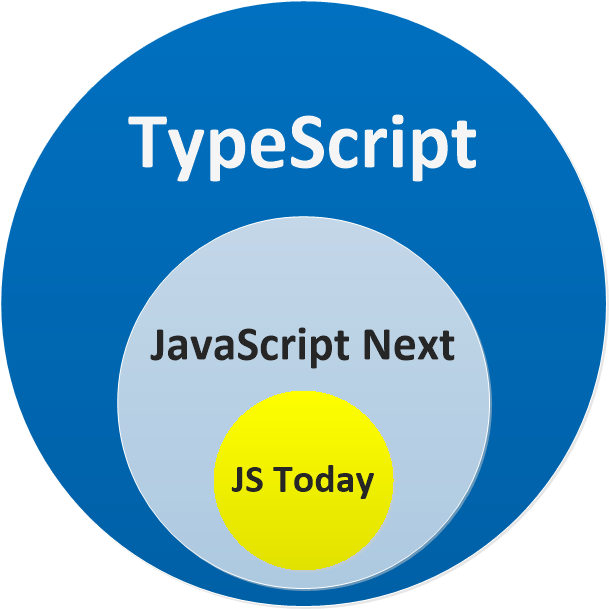
\includegraphics[width=0.6\textwidth]{Figures/TSJSVenn.png}
      \caption{Venn diagram of TypeScript and JavaScript}
      \label{fig:tsjsvenn}
\end{figure}

\begin{multicols}{2}

      \textbf{Algolia}

      Algolia is used for search functionality. It is a search-as-a-service platform that enables developers to
      integrate and build fast, relevant search functionality into their applications and websites (\cite{algolia}).
      It provides a range of features and capabilities for building and managing search functionality, including
      full-text search, typo tolerance, and relevance tuning, as well as analytics and monitoring tools to help
      developers understand how users are interacting with their search functionality in real-time.

      The reason as to why \acrshort{qict} uses Algolia is that the nature of Firebase search engine is quite often
      proven to be inaccurate and slow.

      \textbf{Secret Manager}

      It is a fully managed service provided by \acrshort{gcp} that allows developers and organization to securely store,
      access, and manage sensitive information such as API keys, passwords, certificates, \acrshort{oauth} credentials,
      \acrshort{db} credentials and other credentials used in throughout the lifecycle of their applications
      (\cite{googlesecretmanager}). It is not part of Firebase, and it helps the \acrshort{qaas} app to centralize and
      secure its secrets in scalable and easily manageable way. Key-features of Secret Manager include:
      \begin{itemize}
            \item Secure Storage: it encrypts the secret values using \acrshort{cmek}, ensuring the sensitive data is protected
                  both at rest and in transit.
            \item Audit Logs: it provides and manages audit logs that record all access and modification of activities, helping
                  developers meet compliance, better accountability and regulatory requirements.
            \item Versioning and Automatic Rotation: it supports versioning of secrets, allowing developers to store multiple versions
                  of the same secret. This means that the developers get to keep multiple versions of secrets and easily revert or roll
                  back to a previous version if needed, which will help in auditing and tracking changes to secrets over time. This feature
                  enables automatic seamless rotation of secrets at regular intervals without  disrupting the applications, which improves
                  the security part of the application by ensuring that secrets are regularly updated without manual intervention.
            \item Access Control: it provides fine-grained access control using Google \acrshort{iam}, allowing developers to specify
                  who can access and manage the stored secrets and what they can do with them.
            \item Centralized Management: it stores and manages all secrets in one place, simplifying access and control.
      \end{itemize}
      Cloud Functions can typically access \acrshort{gcp} Secret Manager by....

      \textbf{NoSQL Database}

      is a category of \acrshort{db} that provides a mechanism for storage and retrieval of data that is modelled in ways other
      than the tabular relations used in \acrshort{rdbms}. \acrshort{nosql} \acrshort{db}s are typically designed to handle large
      volumes of unstructured or semi-structured data, such as \acrshort{json}, \acrshort{xml}, or binary objects, and they offer
      a flexible data model that can evolve over time. Both databases in Firebase, Firestore, and Real-time Database are \acrshort{nosql}
      databases. Some characteristics of \acrshort{nosql} \acrshort{db}s include (\cite{nosql}):
      \begin{itemize}
            \item Data Model: \acrshort{nosql} uses dynamic schema, which allows data to be inserted without having to define the schema
                  first, while \acrshort{sql} uses a fixed schema to store data.
            \item Data Structure: \acrshort{nosql} \acrshort{db}s use a variety of data structures such as key-value pairs, document-oriented,
                  graphs databases, and columns-oriented; unlike \acrshort{sql} which only uses tables to store data.
            \item Querying: \acrshort{nosql} uses variety of query languages, such as Mongo\acrshort{db} query language or Cassandra's
                  \acrshort{cql}, while \acrshort{sql} databases only use \acrshort{sql} as the unified language to query data.
            \item Data Consistency and \acrshort{acid} Compliance: databases that are \acrshort{acid} compliant means that they follow a
                  set of rules to ensure that database transactions are processed reliably and securely. \acrshort{sql} databases are a
                  good example of this, while \acrshort{nosql} databases sacrifice some \acrshort{acid} properties in order to achieve
                  higher performance and scalability.
            \item Use Case: \acrshort{nosql} \acrshort{db}s are ideal for applications that need to handle large volumes of data and
                  require high scalability and flexibility, such as social media platforms, real-time analytics, and content management
                  systems.
            \item Scalability: \acrshort{nosql} databases are traditionally designed for horizontal scalability, meaning they can easily
                  scale out multiple servers or clusters to handle volumes of data and high throughput, which is more cost-effective and
                  allows for better scalability. They are well-suited for distributed and cloud-based environments. \acrshort{sql} databases
                  are traditionally designed for vertical scalability, meaning a single server is scaled up with more powerful hardware and
                  power (\acrshort{cpu}, \acrshort{ram}) to a single server. This can become expensive and limit scalability.
      \end{itemize}
      "Serverless Architecture"
\end{multicols}

\begin{figure}[htbp]
      \centering
      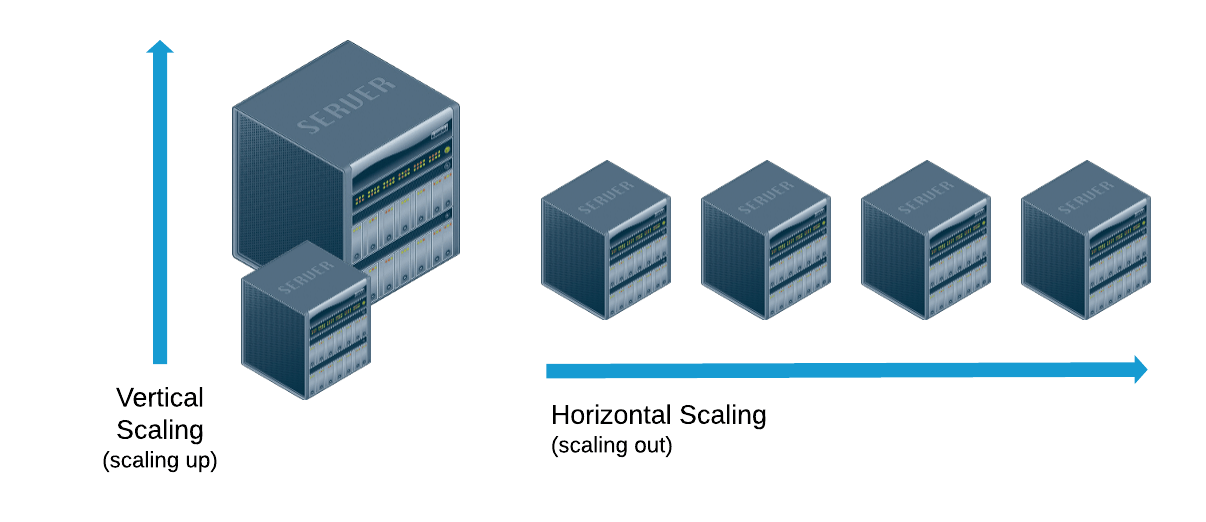
\includegraphics[width=0.8\textwidth]{Figures/nosql-scalling.png}
      \caption{Vertical (\acrshort{sql}) \acrshort{vs} Horizontal (\acrshort{nosql}) Scaling}
      \label{fig:graphqlvsrestarchitecture}
\end{figure}

\begin{multicols}{2}
      Some examples of \acrshort{nosql} databases include Mongo\acrshort{db} (document-oriented), Cassandra (wide-column store), Redis
      (key-value store), and Neo4j (graph database). Some examples of \acrshort{sql} databases include My\acrshort{sql},
      Postgres\acrshort{ql}, and \acrshort{ms} \acrshort{sql} Server.
      \subsection{Q-ICT Internal APIs}
      \subsubsection{What is an API?}
      \acrshort{api} is a software intermediary that allows two applications to talk to each other. They are an
      accessible way to extract and share data within and across organizations.
      \subsubsection{Web APIs}
      A web \acrshort{api} is an \acrshort{api} that can be accessed using the \acrshort{http} protocol. Not all
      \acrshort{api}s are web \acrshort{api}s; some \acrshort{api}s are used only to communicate between two
      applications on the same computer, never making use of a web connection. But in practice, when developers talk
      about \acrshort{api}s, they are almost always talking about web-based \acrshort{api}s used to

      \textbf{JSON format}
      \acrshort{json} is a lightweight data-interchange format that is easy for humans to read and write while being
      also easy for machines to parse and generate too. It is based on a subset of the JavaScript programming language
      and is commonly used for representing structured data. \acrshort{json} is often used for transmitting data between
      a server and a web application, as well as for storing configuration data.

      \acrshort{json} data is organized into key-value pairs, where keys are strings and value can be strings (enclosed
      in double quotes `""`), booleans (`true` or `false`), numbers, objects (unordered collections of key-value pairs
      enclosed in curly braces '{}'), arrays (ordered collections of values enclosed in square brackets '[]'), or null.
\end{multicols}

\begin{lstlisting}[language=JSON, caption=Example of a JSON response, label=lst:jsonresponse]
      {
            "name": "John Doe",
            "age": 30,
            "isStudent": false,
            "cars": [
                  { "name": "Ford", "models": ["Fiesta", "Focus", "Mustang"] },
                  { "name": "BMW", "models": ["320", "X3", "X5"] },
                  { "name": "Fiat", "models": ["500", "Panda"] }
            ],
            "hobbies": ["Reading", "Gaming", "Traveling", "Cooking", "Photography", "Painting", "Gardening"],
            "address": {
                  "street": "Sesame Main Street",
                  "city": "New York",
                  "zip": "10001"
            }
      }
\end{lstlisting}

\begin{multicols}{2}
      \textbf{XML format}
      \acrshort{xml} is a markup language that defines a set of rules for encoding documents in a format that
      is both human and machine-readable. It provides a way to structure data in a hierarchical format using
      tags to define elements and attributes within those elements. It is often used for store, design, and
      representing structured data in a portable and platform-independent way, making it easy to create,
      exchange, and process information between different systems, applications, and platforms.

      \acrshort{xml} documents consist of text-based data enclosed in tags, similar to \acrshort{html}, but
      allows users to define their own customized tags and document structures. This flexibility makes
      \acrshort{xml} suitable for representing a wide variety of data types and structures.

      \acrshort{xml} is often used in various domains such as web services, configuration files, data
      interchange between different software systems, and more.
\end{multicols}

\begin{lstlisting}[language=XML, caption=Example of a XML response, label=lst:xmlresponse]
      <?xml version="1.0" encoding="UTF-8"?>
      <response>
          <status>200</status>
          <message>OK</message>
          <data>
              <user>
                  <id>123</id>
                  <username>johndoe</username>
                  <email>johndoe@example.com</email>
                  <role>user</role>
              </user>
              <user>
                  <id>456</id>
                  <username>janedoe</username>
                  <email>janedoe@example.com</email>
                  <role>admin</role>
              </user>
          </data>
      </response>
\end{lstlisting}

\begin{multicols}{2}
      \textbf{OpenAPI Standard}
      Previously known as Swagger, \acrshort{oas} is a specification for writing a public \acrshort{api}, with
      guidelines for details like endpoint naming conventions, data formats, and error messaging
      (\cite{openapistandard}). The standards required by Open\acrshort{api} and its automation of some tasks
      make it easier for a developer to start working with an \acrshort{api} without needing to read through
      a complex code base. For \acrshort{api} producers, Open\acrshort{api} standard offers access to a wide
      variety of tools based on the standards. \acrshort{api} teams can use these tools to quickly up mock
      servers and create high-quality documentation, among other tasks.
      \acrshort{api}s are generally categorized into different types based on their audience, architecture, and
      protocols (\cite{typesofapi}):
      \subsubsection{Different Types of API By Audience}
      \textbf{Public API}: also called external or Open \acrshort{api}, and as the name suggests it is available
      to everyone. They are open for the public to use and integrate with their applications. Developers can quickly
      implement them using little to no authorization, with few require sign-up and generation of the \acrshort{api} Keys
      to access them. This can make them to not be the best regarding security - just because "public" means expanded
      visibility - but sharing data with them is easier.

      Examples of a public \acrshort{api} are OpenWeatherMap, Google Maps navigation, Facebook and the Twitter \acrshort{api},
      which the latter allows  developers to access Twitter's functionality and data.

      \textbf{Internal API}: also called Private \acrshort{api}, and is used within a private organization to make internal
      apps "talk" to each other. To interact with the data, a developer needs to be actively granted permission to access it,
      because the data and functionality available through the \acrshort{api} are proprietary to the company. They are often
      set up with extensive logging and load-balancing capabilities because they must have greater fault tolerance and
      security than public \acrshort{api}s. They also do not follow the Open\acrshort{api} standard as consistently
      as public \acrshort{api}s, since their producers and consumers typically work together closely, data formats
      can be negotiated based on specific use cases. As they are built by specifically the company; it will only have
      \acrshort{api} protocol types that the organization wants to support. All the \acrshort{api}s managed by the
      \acrshort{qaas} app fall into this category. This solution tend to be very secure, as they are entirely internal.

      \textbf{Partner API}: also called Shared \acrshort{api}, this \acrshort{api} is made considering the scalability
      while developing the business, which will share a few \acrshort{api}s across a few other licensed organizations,
      enabling service offerings across business (\acrshort{b2b}). This \acrshort{api} is shared only with the intended
      users; others might not have access to them because they are not shared publicly, thus making it exists somewhere
      between public and private \acrshort{api}s. They often function to share data between two companies or organizations
      for a specific business purpose, while still ensuring strict privacy protection.

      These \acrshort{api}s indeed require authorization to access them (like having a PayPal account or an \acrshort{api}
      key). All the clients who are part of the business can access and integrate using those \acrshort{api}s. Few
      \acrshort{api}s will only provide read access, and few will provide read/write access via shared \acrshort{api}s.
      This depends on the business process model.

      For example, travel booking \acrshort{api}s are shared with travel agencies to increase their visibility and
      booking. Websites like Expedia, Make My Trip, and Trivago are excellent examples of this kind of \acrshort{api}.

      \subsubsection{Different Types of API Protocols}\label{chap:typesofapis}
      \textbf{\acrshort{soap} \acrshort{api}s}: are strictly based on \acrshort{xml} for the message structure and
      \acrshort{http} for the protocols. \acrshort{soap} itself is a protocol and sending a \acrshort{soap}
      request is similar to using an envelope to send a message. \acrshort{soap} \acrshort{api}s consume extra
      overhead and more bandwidth, and require more work on both the client and server ends. That being said,
      like envelopes, \acrshort{soap} encloses more stringent security compared to \acrshort{rest}. \acrshort{xml}-encoded
      \acrshort{soap} messages use the format defined below:
      \begin{itemize}
            \item \textbf{Envelope}: the root element of the message, which encapsulates the entire
                  \acrshort{soap} message. It 'envelopes' the message by placing tags at the start and the end.
            \item \textbf{Header (optional)}: defines specific additional message requirements, such as authentication.
            \item \textbf{Body}: the request of response is included here.
            \item \textbf{Fault (optional)}: information about errors that might arise during the execution of the
                  \acrshort{api} call or response is highlighted here, along with information on how one can address
                  these errors.
      \end{itemize}
\end{multicols}

\begin{lstlisting}[language=XML, caption=Example of a SOAP request, label=lst:soaprequest]
      <SOAP-ENV:Envelope xmlns:SOAP-ENV="http://schemas.xmlsoap.org/soap/envelope/" xmlns:example="http://example.com">
            <SOAP-ENV:Header/>
            <SOAP-ENV:Body>
                  <example:GetUser>
                        <example:UserID>123</example:UserID>
                  </example:GetUser>
            </SOAP-ENV:Body>
      </SOAP-ENV:Envelope>
\end{lstlisting}

\begin{multicols}{2}
      \textbf{REST API}: if \acrshort{soap} is like an envelope, \acrshort{rest} is like a  more lightweight postcard.
      \acrshort{rest} \acrshort{api}s are considered the gold standard for scalability and are highly compatible with
      microservice architecture. It is the often used protocol in the context of building \acrshort{api}s for web-based
      applications. \acrshort{rest} itself is not a protocol, but an architectural style for designing networked
      applications, defining a set of constraints and principles that define how web services should be structured
      and interact with each other (\textit{see \gls{REST}}).

      \acrshort{api}s that follow \acrshort{rest} principles are called \acrshort{rest}ful \acrshort{api}s. The
      are \acrshort{rest}ful as long as they comply with the 6 guiding constraints of a \acrshort{rest}ful system
      (\cite{restguidingprinciples}):
      \begin{itemize}
            \item \textbf{Client-server architecture}: the architecture is composed of clients, servers, and
                  resources, and it handles requests through \acrshort{http}.
            \item \textbf{Statelessness}: no client is stored on the server between requests. The server should
                  process and complete each request independently. Information about the session state is, instead,
                  held with the client. The clients can do this via query parameters, headers, \acrshort{uri}s,
                  request body, \acrshort{etc}
            \item \textbf{Cacheable}: simply, the clients should be able to determine whether this response is cacheable
                  from their side, and if so, for how long. If a response is cacheable, the client has the right to return the
                  data from its cache for an equivalent request and specified period, without sending another request to the
                  server. A well managed caching mechanism can eliminate the need for some client-server interactions
            \item \textbf{Layered system}: client-server interactions can be mediated by additional layers. These
                  layers could offer additional features like load balancing, shared caches, or security.
            \item \textbf{Uniform interface}: this is the core to design \acrshort{rest}ful \acrshort{api}s.
                  There should be a uniform and standard way of interacting with a given server for all client
                  types. The uniform interface helps to simplify the overall architecture of the system. This includes
                  4 facets:
                  \begin{itemize}
                        \item Resource identification in request: resources are uniquely identified in requests and are separate
                              from the representations that are returned to the client using \acrshort{uri}.
                        \item Resource manipulation through representations: clients receive files of a uniform that represent resources.
                              These representations must have enough information to allow modification or deletion of the resource's
                              state in the server, as long as they have the required permissions.
                        \item Self-descriptive messages: each message returned to a client contains enough information to describe
                              how the client should process the information further, such as additional actions that can be
                              performed on the resource.
                        \item Hypermedia as the engine of application state: after accessing a resource, the \acrshort{rest} client
                              should be able to discover through hyperlinks all other actions that are currently available.
                  \end{itemize}
            \item \textbf{Code on demand (optional)}: servers can extend the functionality of a client by transferring
                  executable code.
      \end{itemize}
      \acrshort{rest} \acrshort{api}s are high-performing (especially over \acrshort{http}2), time-tested, and support
      many data formats. They also decouple the client and server, making sure of independent evolution. However,
      building a true \acrshort{rest} \acrshort{api} is difficult because it requires a disciplined adherence to the
      Uniform Interface constraint (\cite{restapiuniforminterface}). Some organizations trade off the long-term benefits
      of a truly \acrshort{rest} \acrshort{api} for other \acrshort{http} \acrshort{api} protocols that have similar
      benefits but adhere to \acrshort{rest} constraints more liberally. \acrshort{rest} requests typically include these
      key components:
      \begin{itemize}
            \item \textbf{Endpoint}: the uniform resource identifier that locates the resource on the internet is
                  part of this component. \acrshort{url}s are the most common type of \acrshort{uri}.
            \item \textbf{HTTP Method}: this component outlines the four basic processes that a resource can be subjected
                  to: POST (create a resource), GET (retrieve a resource), PUT (update a resource), and DELETE
                  (remove a resource).
            \item \textbf{Headers}: data related to the server and the client are stored in this component. Like in
                  \acrshort{soap}, one can also use \acrshort{rest} headers to store authentication measures such as
                  \acrshort{api} keys, server \acrshort{ip} addresses, and the response format.
            \item \textbf{Body}: this component contains additional information for the server, such as data that needs to
                  be added or replaced.
      \end{itemize}
\end{multicols}
\begin{lstlisting}[language=JavaScript, caption=Different HTTP methods in REST]
            GET /users <@\textnormal{Retrieve list of all users}@>
            GET /users/{id} <@\textnormal{Retrieve details a specific user by their ID}@>
            POST /users <@\textnormal{Create a new user}@>
            PUT /users/{id} <@\textnormal{Update a specific user by their ID}@>
            DELETE /users/{id} <@\textnormal{Delete a specific user by their ID}@>
\end{lstlisting}
\begin{lstlisting}[language=JavaScript, caption=REST's Example Request]
            GET https://api.example.com/users/123
\end{lstlisting}
\begin{lstlisting}[language=JavaScript, caption=Example of REST request in JavaScript]
      const apiUrl = 'https://api.example.com/users/123';

      // Define the request parameters
      const requestOptions = {
            method: 'GET', // HTTP method (GET, POST, PUT, DELETE, PATCH, etc.)
            headers: {
                  'Content-Type': 'application/json', // Set the content type of the request
            }
      };

      // Make the API request
      fetch(apiUrl, requestOptions)
            .then(response => response.json())
            .then(data => console.log(data)) // Process the response data
            .catch(error => console.log('error', error)); // Handle any errors that occurred during the request
\end{lstlisting}
\begin{multicols}{2}
      All three of the \acrshort{rest}, \acrshort{soap}, and Graph\acrshort{ql} use the \acrshort{http} protocol for
      communication therefore falls into \acrshort{http} \acrshort{api}s category. They are the commonly used for web
      services  and allow applications to interact with each other over the internet. \acrshort{http} is superbly
      suited for applications following a request-response paradigm.
\end{multicols}

\begin{multicols}{2}
      With that being said, the \acrshort{qaas} app needs to manage and make connection different sort of \acrshort{api}s.
      Those \acrshort{api}s are the following:
      \begin{itemize}
            \item Resello: is used for \acrshort{qict} \acrshort{ms} subscriptions owned by Pax8. It is a cloud
                  marketplace that simplifies the way \acrshort{sme}s buy, sell, and manage cloud solutions through
                  automation. It provides a single platform to manage the entire cloud customer lifecycle, from
                  quote to cash to support, thus simplifying the process of buying, selling and managing cloud
                  solutions.
            \item SnelStart: is used for \acrshort{qict} automation of financial and accounting system software,
                  such as managing invoices, \acrshort{etc} for \acrshort{sme}s. It offers a range of products and
                  services to help businesses manage their finances, including accounting software, invoicing software,
                  and financial management tools.
            \item Bodyguard.io: is a \acrshort{cdr} tool used for security tab. It is a product from a Dutch company
                  that filters and scrutinizes downloads from web browsers to detect and prevent malicious files with
                  real-time download scanning capabilities.
            \item N-Central: is a product from N-Able and is used for monitoring clients' devices and ensuring the
                  overall security of their systems, \acrshort{it} infrastructure, and digital assets. It is a
                  \gls{RMM} platform designed to help \acrshort{msp} and \acrshort{it} professionals to
                  remotely monitor and manage their clients' devices and networks. It provides a comprehensive
                  set of tools and features for monitoring, managing, and securing clients' devices and networks,
                  including remote monitoring and management, patch management, antivirus, backup and disaster
                  recovery, and network topology mapping. The return response from this \acrshort{api} is in \acrshort{xml}
                  and \acrshort{json} format, making it both a \acrshort{rest} and \acrshort{soap} \acrshort{api}.
      \end{itemize}
      \section{Research Sub-Question \#2}
      \subsection{SentinelOne} % vs CrowdStrike with Carbanak and FIN7 methodology, Huntresss, datto rmm
      To answer this research sub-question, a general understanding of what SentinelOne is needed in order to know what
      methods should be utilized to integrate it with the \acrshort{qaas} app.

      SentinelOne is a cybersecurity platform that provides endpoint protection, detection, and response capabilities to
      help organizations defend against advanced cyber threats. It leverages \acrlong{ai} and machine learning to analyze
      and respond to security threats in real-time, providing organizations with comprehensive protection against malware,
      ransomware, and other cyber threats. It also provides visibility into clients' \acrshort{it} systems and infrastructure,
      enabling organizations to gain insights into potential security risks and vulnerabilities and take proactive measures
      to address them.

      Some terminology that the readers need to be familiar with before diving deeper into SentinelOne:

      \textbf{Endpoint}

      Endpoint can be defined as any remote computing devices that receives incoming communications and sends outgoing messages
      to the network it is connected to. Examples of endpoints include desktops, laptops, smartphones, tablets, servers, workstations,
      and other \acrshort{iot} devices that is connected to a network. They are the first-line of defence for the Blue team today.

      \textbf{EPP}

      \textbf{EDR}

      \acrshort{edr} \acrshort{aka} \acrshort{etdr}, is a group of integrated endpoint security solutions that combine data collection,
      data analysis, forensics, and threat hunting with the end-goal of identifying and stopping any potential security breaches in due time.
      \acrshort{edr} solutions are able to recognize any suspicious patterns that can be investigated later on, as they have been purposefully
      created to detect and respond in an active manner to advance malware, ransomware, and other cyber threats (the Response \acrshort{edr}).
      \acrshort{edr}, as the name suggest, were developed specifically for endpoints, and not networks (\ref{sec:ndr}).

      The number one thing that sets apart \acrshort{edr} from traditional \acrshort{av} is that traditional \acrshort{av} relies on
      signature-based detection, usually having a defined set of list in their \acrshort{db}, where known malware signatures are compared
      against files or processes to identify threats. \acrshort{edr} on the other hand, uses a combination of signature-based detection, such
      as behavioural analysis, machine learning, and anomaly detection to identify and respond both known and unknown threats. \acrshort{edr}
      solutions focus on detecting malicious activities at the endpoint level, including file modifications, process execution, and network
      connections, focusing on malicious behaviour compare to only concerning with malicious software like what traditional \acrshort{av} does.

      \textbf{MDR}

      \textbf{NDR} \label{sec:ndr}

      \textbf{SIEM}

      is a software system that collects, aggregates, normalizes security data from a variety of sources within an IT infrastructure, and
      analyzes it according to pre-set rules, present it in human-readable format and therefore giving a comprehensive picture of the company's
      information security. \acrshort{siem} tools evolved from the log management discipline and combine \acrshort{sim} and \acrshort{sem} technologies.
      A \acrshort{siem} tool uses \acrshort{ai} to automate a number of manual procedures related to threat detection and incident response. Furthermore,
      it assists enterprise security teams in spotting anomalies in user behavior.

      \begin{itemize}
            \item Input: logs, threat intel, vulnerability feeds, \acrshort{ndr}, and \acrshort{edr} data
            \item Output: high-fidelity alerts prioritized by severity
            \item Infused with: \acrshort{ai}, \acrshort{ml}, and analytics
      \end{itemize}

      \textbf{XDR}

      is a security solution that gathers and analyzes data from multiple sources like endpoints, networks, cloud, emails, app, \acrshort{etc} It offers
      great visibility into a company's \acrshort{it} infrastructure, helping the security employees to detect more threats, respond efficiently, and
      deal with fewer false positive alerts \cite{xdrIDC}.

      This solution integrates several tools combining all the gathered data into a single platform to visualize the information. It might incorporate
      automated processes (even complex ones), \acrshort{ml}, and advanced analytics to enable quicker and more effective incident response. It can
      deal even with hidden and advanced malware.

      \textbf{MXDR}

      Some people still call it \acrshort{mdr}, managed \acrshort{soc}, or managed security.

      \textbf{SOAR}

      \acrshort{soar} solutions focus on automating incident response processes and triage capabilities. The main goal is to oversee security without
      human help as much as possible, boosting productivity and shorten the response time. It might use \acrshort{ai} and \acrshort{ml} to assess
      security events and automate incident response procedures. These solutions can be standalone product, or it can be added to \acrshort{siem}
      solutions since \acrshort{soar} does not excel in event analysis.

      \textbf{SOC}

      \begin{figure}[htbp]
            \centering
            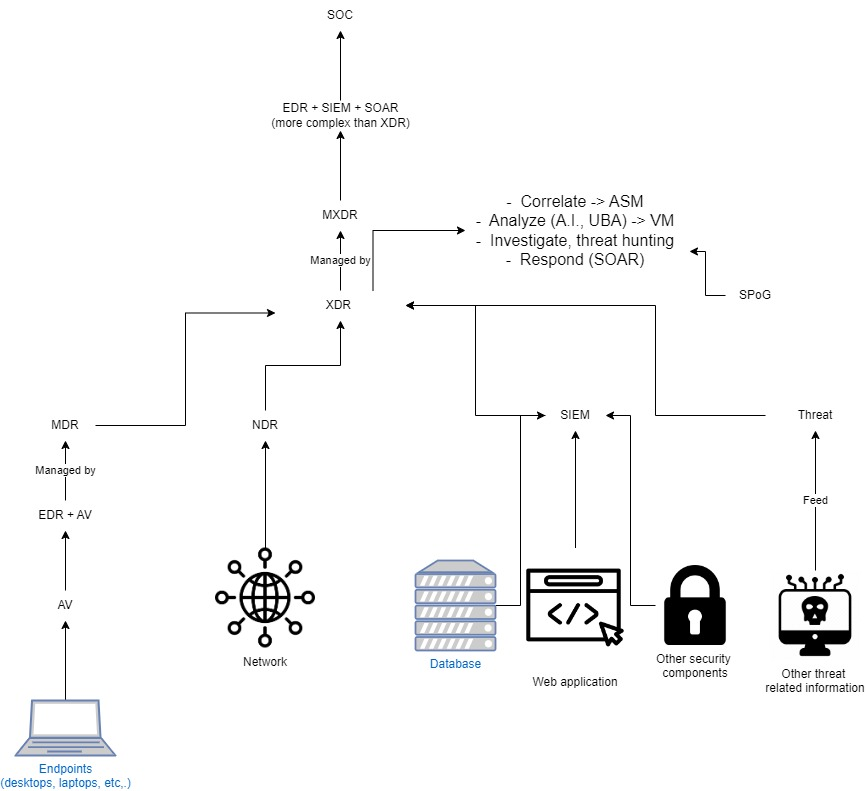
\includegraphics[width=0.6\textwidth]{Figures/XDR.jpg}
            \caption{How all terms related to various technologies in cybersecurity connected to each other}
            \label{fig:xdr}
      \end{figure}

      \textit{Please note that as mentioned before, \acrshort{siem} can also take data from an \acrshort{edr} and \acrshort{ndr} but for
            the sake of simplicity, the diagram puts them as a separate pier systems.}

      \subsection{SentinelOne Console}

      \subsection{SentinelOne Agent}
      An Agent is a software program, deployed to each endpoint, including desktop, laptop, server or virtual environment,
      and runs autonomously on each device, without reliance on Internet connection, enabling data gathering, detection, and
      response to actions. Agents can be interpreted as an \acrshort{av}, collecting relevant security telemetry such as:
      \begin{itemize}
            \item Running processes
            \item Connected servers
            \item Open files
      \end{itemize}
      This information can be useful to detect the presence of a threat or to use in forensic analysis and investigation after
      an attack has occurred (Recovery).
      \subsection{Ranger}
      Ranger is one of the SentinelOne product that provides a way of detecting other devices (computers and
      \acrshort{iot} devices) that are on the client's computer network. If a malicious attacker comes in and plugs his device
      into the network, all the other SentinelOne agents are going to read the network traffic, determine and classify whether
      this is a new device, or a rogue device. As long as a device has Ranger on that network subnet, SentinelOne can gather and
      detect technical information regarding the device. On a network, before a machine is connected and talks to other devices
      and gateways, it is going to do a broadcast and gives up information about itself. This is called an \acrshort{arp} request.
      Ranger is going to read that \acrshort{arp} request and determine
      \subsection{Sentinels}
      Sentinels are the end-points,

      \subsection{Incidents}

      \begin{itemize}
            \item Kill: stops all processes related to that threat
            \item Quarantine: encrypts and moves the threat and its executables
            \item Remediate: deletes all files and system changes created by the threat
            \item Rollback: restores files and configuration that the threat changed. This step is usually taken when a malware has
                  executed its script and has made changes to the system, \acrshort{eg} a ransomware has encrypted all the files and
                  asked for a ransom. By executing this step, all the three previous steps will also be undertaken as well. This will
                  then reboot the system and restore it to the safe state before the malware has executed.
      \end{itemize}

      Additionally, the user can also perform an analysis verdict
      \begin{itemize}
            \item False positive
            \item Suspicious
            \item True positive
            \item Undefined
      \end{itemize}

      Threat mitigation status
      \begin{itemize}
            \item Mitigated
            \item Not mitigated
            \item Marked as benign
      \end{itemize}

      Incident status
      \begin{itemize}
            \item Resolved
            \item Unresolved
            \item In progress
      \end{itemize}

      \acrshort{ai} confidence Level
      \begin{itemize}
            \item Malicious
            \item Suspicious
            \item \acrshort{na}
      \end{itemize}

      Classification
      \begin{itemize}
            \item Malware
            \item \acrshort{pua}
            \item Virus
            \item Infostealer
            \item Hacktool
      \end{itemize}

      \acrshort{os}
      \begin{itemize}
            \item Windows
            \item Linux
            \item Mac
            \item Windows Legacy
      \end{itemize}

      Cloud Provider
      \begin{itemize}
            \item Azure
            \item \acrshort{aws}
            \item \acrshort{gcp}
            \item \acrshort{oci}
            \item ESXI
      \end{itemize}

      Engine
      \begin{itemize}
            \item SentinelOne Cloud
            \item On-Write Static \acrshort{ai} - Suspicious
            \item Behavioral \acrshort{ai}
            \item On-Write Static \acrshort{ai}
            \item Reputation
            \item Cloud Detection
            \item User-Defined Blocklist
            \item Documents, Scripts
            \item Anti Exploitation / Fileless
            \item Intrusion Detection
            \item Potentially unwanted application
            \item Lateral Movement
            \item Remote Shell
            \item Manual
            \item Application Control
            \item Threat Intelligence
            \item WatchTower
            \item Driver Blocking
      \end{itemize}

      Initiated by:
      \begin{itemize}
            \item Agent Policy
            \item Full Disk Scan
            \item Local agent command
            \item Deep Visibility Command
            \item Management console \acrshort{api}
            \item On-Demand Scan
            \item Custom Rule
            \item Custom Alert
            \item Cloud Detection
            \item Threat Intelligence
            \item WatchTower
      \end{itemize}

      Additionally, users can also search the mitigated threats by:
      \begin{itemize}
            \item Content Hash
            \item Cloud Account
            \item Cloud Image
            \item Cloud Instance \acrshort{id}
            \item Cloud Instance Size
            \item Cloud Location
            \item Cloud Network
            \item \acrshort{aws} Role
            \item \acrshort{aws} Security Groups
            \item \acrshort{aws} Subnet \acrshort{id}s
            \item Azure Resource Group
            \item \acrshort{gcp} Service Account
            \item Threat Details: \acrshort{eg}: "This is a non-Microsoft binary that masquerades as a Microsoft executable"
            \item File Path: \acrshort{eg}: "\textbackslash Device\textbackslash HarddiskVolumeA\textbackslash Users\textbackslash Chris\textbackslash Downloads\textbackslash malicious.exe"
            \item Endpoint Name" \acrshort{eg}: "LT-Christopher", "LT 10-08"
            \item \acrshort{uuid}: \acrshort{eg}: "0ff2a3409f284776a23432e9f6894afa"
            \item Agent Version (at detection): \acrshort{eg}: "23.1.4.650"
            \item Agent Version (current)
            \item Domain (at detection time)
            \item Command Line Arguments
            \item Initiated By (username): \acrshort{eg}: "LuukAdmiraalMKBIT"
            \item Storyline
            \item Originated Process
            \item Cluster Name
            \item Node Name
            \item Namespace Name
            \item Namespace Labels
            \item Controller Name
            \item Controller Labels
            \item Pod Name
            \item Pod Labels
            \item Container Name
            \item Image Name
            \item Container Labels
            \item External Ticket \acrshort{id}
            \item Node Labels
      \end{itemize}

      Furthermore, it will also analyze for infected endpoint connectivity (offline/online), mitigated preemptively (yes/no),
      reboot required (yes/no), action failed (yes/no), pending actions (yes/no), and if note and external ticket exists (yes/no).
      \subsection{Reports}
      \subsection{Vigilance}
      It is a \acrshort{mdr} service - providing threat monitoring, hunting, and response, to its existing customers. It
      provides a 24/7 \acrshort{soc} with expert analysts and researchers to give customers near real-time threat monitoring,
      in-console threat annotations, and response to threats and suspicious events. Vigilance itself is a separate package from
      SentinelOne.
      \section{Research Sub-Question \#3}
      Please keep in mind that in this sub-question, only the visualization techniques will be assessed, compared, contrasted,
      evaluated, and discussed. The other factors such as pricing, technologies, and features will not be discussed in this sub-question.
      \subsection{Heimdal\textregistered}
      \subsection{Huntress}
      \subsection{CrowdStrike}
      CrowdStrike Falcon
      \subsection{Datto RMM}
      \subsection{Sophos}
      \subsection{Carbon Black}
      \subsection{Trend Micro}
      Trend Micro Apex One
      \subsection{Kaspersky Endpoint Security}
      \subsection{Bitdefender}
      Bitdefender Gravity Zone
      \subsection{McAfee}
      \subsection{Symantec}
      \subsection{Trend Micro}
      \subsection{Cynet 369}
      \subsection{Microsoft Defender for Endpoint}
      \section{Research Sub-Question \#4}
\end{multicols}